\documentclass{article}

\usepackage[utf8]{inputenc}
\usepackage[T1]{fontenc}      
\usepackage[francais]{babel}
\usepackage{graphicx}
\usepackage{circuitikz}
\usepackage[squaren, Gray]{SIunits}
\usepackage{sistyle}
\usepackage[autolanguage]{numprint}
\usepackage{pgfplots}
\pgfplotsset{compat=1.9}
\usepackage{amsmath,amssymb,array}
\usepackage[top=2.5cm,bottom=2.5cm,right=2.5cm,left=2.5cm]{geometry}
\usepackage{url} 
\usepackage{tabularx}
\DeclareMathOperator{\dist}{d}
\newenvironment{abstract-fr}
{
	\begin{center}
		\textbf{Résumé} \\[0.5cm]
	\end{center}
}
{}

\newenvironment{abstract-en}
{
	\begin{center}
		\textbf{Summary} \\[0.5cm]
	\end{center}
}
{}
% New command pour la modélisation mécanique, tri à effectuer
\newcommand\fv[1]{{\bf #1}} % free vector
\newcommand\fvd[1]{\dot{\bf #1}} % free vector derivated
\newcommand\fvdd[1]{\ddot{\bf #1}} % free vector derivated
\newcommand\fvr[1]{\mathring{\bf #1}} % free vector relatively derivated
\newcommand\fvrr[1]{\overset{\circ\circ}{\bf #1}} % free vector relatively derivated
\newcommand\uv[1]{{\bf\hat{ #1}}} % unit vector
\newcommand\ui{{\bf\hat{I}}} % unit vector I
\newcommand\uj{{\bf\hat{J}}} % unit vector J
\newcommand\uk{{\bf\hat{K}}} % unit vector K
\newcommand\wrt[2]{\ensuremath{\tensor*[_{ #1}]{ #2}{}}} % With Respect To
\newcommand\wtr[3]{\ensuremath{\tensor*[_{ #1}]{ #2}{^{ #3}}}} % With Two Respect
\newcommand\omegaf{{\bm \omega}}
\newcommand\omegafr{\mathring{\bm \omega}}
\newcommand\omegafd{\dot{\bm \omega}}
\newcommand\omegaft{\tilde{\bm \omega}}
\newcommand\omegaftr{\mathring{\tilde{\bm \omega}}}
\newcommand\omegat{\tilde{\omega}}
\newcommand\omegatd{\tilde{\dot{\omega}}}
\newcommand\ine{{\bf I}}
\newcommand\st{{\bf L}}
\newcommand\pst{{\bf M}}
\newcommand\lm{{\bf N}}
\newcommand\am{{\bf H}}
\newcommand\amd{\dot{\am}}
\newcommand\fo{{\bf F}}
\newcommand\po{\mathcal{P}}
\newcommand\xg{\ensuremath{\fv{R}}}
\newcommand\xgd{\ensuremath{\fvd{R}}}
\newcommand\xgdd{\ensuremath{\fvdd{R}}}
\newcommand\dvec[1]{\dot{\vec{ #1}}}
\newcommand\ddvec[1]{\ddot{\vec{ #1}}}
\newcommand\qp{\dot{q}}
\newcommand\dqp{\Delta \dot{q}}
\usepackage{url} 
\usepackage{hyperref}
\hypersetup{
    colorlinks,
    citecolor=black,
    filecolor=black,
    linkcolor=black,
    urlcolor=black
}

\begin{document}

\section{Fonctionnement général}
% Description générale du système + concepts physiques clés
Notre haut-parleur peut-être représenté schématiquement comme sur la Figure \ref{block-diagram-hp}.

% Schéma montrant le bonne compréhension du système
\begin{figure}[!htb]
	\centering
	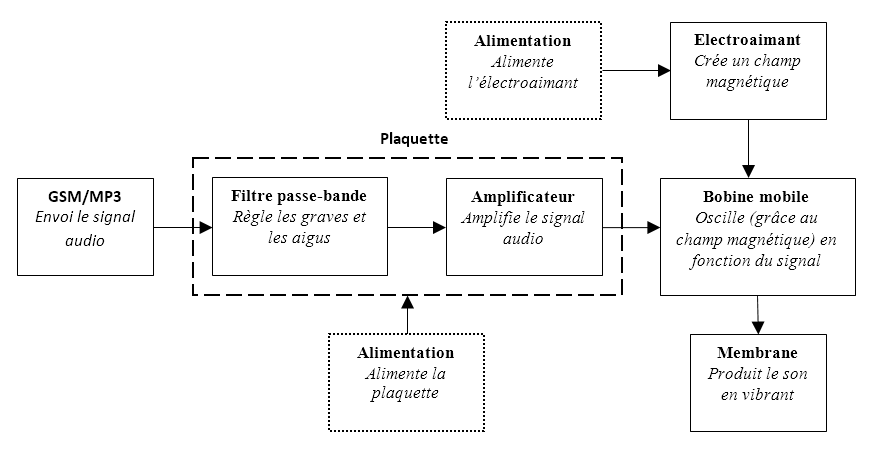
\includegraphics[scale=0.68]{schema_fonctionnel.png}
	\caption{Schéma fonctionnel du haut-parleur.}
	\label{block-diagram-hp}
\end{figure}

Le GSM ou le MP3 va dans un premier temps envoyé un signal audio via le cable Jack au circuit
imprimé, par la suite nous qualifierons ce signal de \textit{brut}. Le circuit imprimé permet
quant à lui de modifier ce signal brut de plusieurs façon : 

\begin{itemize}
	\item En règlant le volume, c'est à dire en modifiant l'amplitude du signal audio ;
	\item En règlant les graves et les aigus, c'est à dire en atténuant les basses fréquences
	(rôle du filtre passe-haut, circuit CR) ou les hautes
	fréquences (rôle du filtre passe-bas, circuit RC). Il s'agit du rôle des filtres passe-bas 
	et passe-haut qui combiné forme un filtre passe-bande ;
	\item En amplifiant le signal : c'est le rôle de l'amplificateur audio du circuit.
\end{itemize}

A la sortie du circuit imprimé, le signal est alors \textit{filtré} et \textit{amplifié}.
Ce signal traité ira ensuite alimenter en courant la bobine mobile. Cette 
dernière intercepte un champ magnétique constant, noté $B$, produit par l'électroaimant.
L'électroaimant est constitué de fines lamelles de matériau magnétique en forme de ''E'' 
empilé les unes sur les autres. La perméabilité magnétique élevé de ce matériau
($\mu_r \approx \ 1600$) permet de créer un champ magnétique plus fort. Autour de la branche
centrale du ''E'' est enroulée du fil de cuivre, formant ainsi une bobine.
% Premier concept physique, loi d'Ampère
Le champ magnétique $B$ produit par l'électroaimant dans l'entrefer peut être calculer par la 
loi d'\textsc{Ampère} :

$$\vec{B} = \mu_0\mu_r\frac{NI}{e}$$

Où $N$ est le nombre de spires, $I$ le courant traversant la bobine et $e$ la largeur de 
l'entefer.

% Deuxième concept physique, force de Laplace
La bobine mobile subit donc une force de \textsc{Laplace} dont l'expression est :

$$\vec{F} = i(t)\vec{L}\times{\vec{B}}$$ 

Où $L$ est la longueur du fil et$i(t)$ le courant le traversant. Cette force est proportionnelle
au courant traversant
la bobine mobile. La membrane se déplacera donc de manière cohérente avec le signal audio
et reproduira le son voulu. Enfin, la membrane pourra revenir à son position d'équilibre
grâce à des attaches qui, à la manière de ressorts, produisent une force de rappel dans la
direction opposée au mouvement de la bobine mobile :

$$\vec{F} = -kx$$ % Troisième concept physique, loi d'Hook

Ou $k$ est la constante de raideur des attaches et $x$ est le déplacement de la bobine mobile
par rapport à sa position d'origine (et donc la compression des attaches).

\paragraph{Remarque}
Une description plus détaillée de chaque composants du circuit électriques est présentée
dans l'annexe ''Analyse séquentielle du circuit''.

% Just here to fix rapport_prejury.tex
\end{document}